\subsection{Sparse Readout Prism}
\label{sec:method-srp}

Sparse Readout Prism (SRP) provides a sparse coordinate system for the final
readout. Rather than explaining logits only in the vocabulary-row basis, SRP
factorizes unembedding rows into sparse token-specific coefficients and shared
decoder directions in hidden-state space. This yields three linked objects: a
reconstructed LM head for global faithfulness checks, a target-independent
profile \(D_{\mathrm{feat}}h\) describing which readout features are present in
a hidden state, and, once a scalar readout target is fixed, a local signed
account of that score with an explicit residual. Here, \emph{local} means
conditioned on both a hidden state \(h\) and a scalar target \(q_\alpha\). All
score decompositions below are evaluated after mapping SAE quantities back to
the model's raw readout coordinates.

\begin{figure}[t]
    \centering
    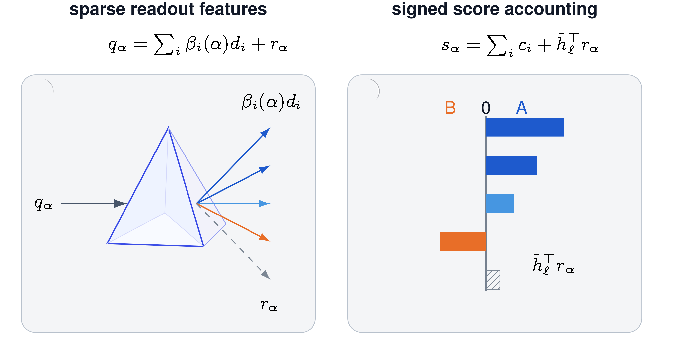
\includegraphics[width=\columnwidth]{figures/schematic_tikz/readout_query_one_column.pdf}
    \vspace{-0.8\baselineskip}
    \caption{\textbf{Local score account schematic.}
    A centered or contrast readout target is decomposed into SAE features learned
    from unembedding rows. For \(w_A-w_B\), \(A\) and \(B\) are the competing
    token or token-set sides: positive bars support \(A\) over \(B\), negative bars
    support \(B\) over \(A\). At hidden state \(h\), each signed term is a target
    coefficient times \(h\)'s feature projection; hatching marks reconstruction
    error. Raw token-logit targets also include a shared offset.}
    \label{fig:readout-query-schematic}
\end{figure}

\subsubsection{SAE Over Unembedding Rows}

For each token row \(t\), the readout SAE approximates the corresponding
unembedding vector. In the raw readout coordinates used for all score accounts,
the fitted row and residual satisfy
\[
    \widehat{w}_t = \mu + \sum_{i=1}^{D} z_{t,i} d_i,
    \qquad
    r_t = w_t-\widehat{w}_t,
\]
where \(\mu\) is a shared offset, \(d_i\in\R^d\) is a decoder direction,
\(z_{t,i}\) is the sparse coefficient of token row \(t\), and \(r_t\) denotes
the residual. Thus the row identity used below is
\[
    w_t=\mu+\sum_i z_{t,i}d_i+r_t .
\]
The explicit residual is the only approximation term in later score
decompositions.
Stacking the fitted rows \(\widehat{w}_t^\top\) yields
\(\widehat{\WU}\). Appendix~\ref{app:score-accounting} provides details on
centering and row normalization.

The reported TopK models first center, and optionally row-normalize, the
readout rows:
\[
    x_t = \frac{w_t-\mu}{a_t},
\]
where \(a_t=1\) when row normalization is not used. An encoder produces a
\(D\)-dimensional pre-code, retains the \(k\) largest entries, and decodes the
result using directions \(\widetilde d_i\):
\[
    \widetilde z_t
    =
    \operatorname{TopK}_k(f_\theta(x_t)),
    \qquad
    \widehat{x}_t
    =
    \sum_{i=1}^{D}\widetilde z_{t,i}\widetilde d_i .
\]
The objective is row reconstruction,
\[
    \min_{\theta,\{\widetilde d_i\}}
    \frac{1}{|\mathcal{V}|}
    \sum_{t\in\mathcal{V}}
    \left\|x_t-\widehat{x}_t\right\|_2^2 .
\]
After fitting, we convert the learned representation back to raw readout
space by setting
\[
    z_{t,i}=a_t\widetilde z_{t,i},
    \qquad
    d_i=\widetilde d_i,
    \qquad
    r_t=a_t(x_t-\widehat{x}_t).
\]
Consequently, all subsequent decompositions are expressed in terms of the
model's original logits or contrasts, with no additional dense correction term.
The width \(D\) and native sparsity \(k\) are selected using held-out
reconstruction quality and readout-replacement fidelity.
Appendices~\ref{app:readout-factorizer-sweeps}--%
\ref{app:readout-factorizer-diagnostics-reproducibility} provide the selection
procedure, recipe sweeps, transfer rows, diagnostics, and reproducibility
details.


\subsubsection{Full Readout Replacement and Profiles}

The same factorization can be applied to the whole readout map. Let \(Z\in
\R^{|\mathcal{V}|\times D}\) collect the sparse row codes and let
\(D_{\mathrm{feat}}\in\R^{D\times d}\) have rows \(d_i^\top\). Then
\[
    \begin{aligned}
    \widehat{\WU}
    &=
    \mathbf{1}\mu^\top
    +
    ZD_{\mathrm{feat}},\\
    \widehat{\ell}(h)
    &=
    \widehat{\WU}h\\
    &=
    \mathbf{1}(\mu^\top h)
    +
    Z(D_{\mathrm{feat}}h).
    \end{aligned}
\]
The vector \(D_{\mathrm{feat}}h\) is the target-independent \emph{profile}: it
records which learned readout directions are present in \(h\) before any token
or contrast has been selected. A profile coordinate is not evidence by itself;
it becomes support or opposition only after multiplication by a row code or
target coefficient. We use full readout replacement to measure global
faithfulness of the factorization, and the local contributions below to measure
target-conditioned accounts.

We use TopK readout SAEs \citep{makhzani2013ksparse,gao2024scaling}; all
quantitative reconstructions use the full feature sum, while visualizations may
truncate small bars for readability.

\subsubsection{Local Score Decomposition}

Fix a hidden state \(h\) and any scalar readout target
\(q_\alpha=\sum_{t\in\mathcal{V}}\alpha_t w_t\), substituting the SAE
reconstruction gives
\[
\begin{aligned}
    s_\alpha(h)
    &= h^\top q_\alpha \\
    &=
    \left(\sum_{t\in\mathcal{V}} \alpha_t\right) h^\top\mu \\
    &\quad + \sum_{i=1}^{D}
        \left(\sum_{t\in\mathcal{V}} \alpha_t z_{t,i}\right) h^\top d_i \\
    &\quad + h^\top \sum_{t\in\mathcal{V}} \alpha_t r_t .
\end{aligned}
\]
For SAE feature \(i\), define its coefficient for the chosen target and its
Sparse Readout Prism contribution as
\[
    \beta_i(\alpha)=\sum_{t\in\mathcal{V}} \alpha_t z_{t,i},
    \qquad
    c_i(h,\alpha)=\beta_i(\alpha)\,h^\top d_i.
\]
The coefficient \(\beta_i(\alpha)\) is fixed by the target and readout SAE, while
\(h^\top d_i\) changes with context. When \(q=q_\alpha\) is clear, we write
\(\beta_i(q)\). This product form is the central separation in SRP: the
readout-side factor \(\beta_i(q)\) states how feature \(i\) enters the selected
target, while the context-side factor \(h^\top d_i\) states how strongly the
current hidden state projects onto that readout direction. A feature matters
locally when both factors are large. Positive terms raise the chosen scalar;
negative terms lower it. The projection alone belongs to the profile
(Appendix~\ref{app:global-readout-feature-activations}); target coefficients
turn profile activations into token- or contrast-specific evidence.

Let \(s_\mu=(\sum_t\alpha_t)h^\top\mu\),
\(s_{\mathrm{feat}}=\sum_i c_i(h,\alpha)\), and
\(s_{\mathrm{recon}}=s_\mu+s_{\mathrm{feat}}\). The reconstruction error is
\[
    \epsilon
    =
    s_{\mathrm{exact}}-s_{\mathrm{recon}}
    =
    h^\top\sum_{t\in\mathcal{V}}\alpha_t r_t .
\]
This residual is the faithfulness diagnostic for an individual local account:
when \(|\epsilon|\) is small, the displayed feature bars account for the chosen
score; when it is large, the sparse account is incomplete. Figures report the
original target score, feature sum, offset when present, and reconstruction
error alongside contribution bars. For signed contrasts, sign-preserved
reconstructions give directly readable support and opposition.
Appendix~\ref{app:score-accounting} states the full identities.

\subsubsection{Common Target Coefficients}

The same identity covers the target families from \Cref{sec:problem-setup}.
\Cref{tab:method-special-cases} lists \(\beta_i(\alpha)\) for the target
families used in the results.
For compactness, write
\(\bar{z}_{\mathcal{A},i}=|\mathcal{A}|^{-1}\sum_{a\in\mathcal{A}}z_{a,i}\)
for the uniform average of feature \(i\)'s sparse coefficient over token group
\(\mathcal{A}\). For top-competitor margins, write
\(\bar{w}_{\pi,\mathcal{R}}=\sum_{r\in\mathcal{R}}\pi_r w_r\) and
\(\bar{z}_{\pi,\mathcal{R},i}=\sum_{r\in\mathcal{R}}\pi_r z_{r,i}\).

\begin{table}[tbp]
\caption{\textbf{Scalar readout target coefficients.}
Rows instantiate the general target \(q_\alpha\) and corresponding SAE feature
coefficient \(\beta_i(\alpha)\). Barred quantities denote uniform token-set
averages or competitor-weighted averages.}
\label{tab:method-special-cases}
\centering
\footnotesize
\setlength{\tabcolsep}{3pt}
\renewcommand{\arraystretch}{1.14}
\begin{tabularx}{\linewidth}{@{}>{\RaggedRight\arraybackslash}p{0.34\linewidth}Z Z@{}}
\toprule
Target & \(q_\alpha\) & \(\beta_i(\alpha)\) \\
\midrule
\textbf{Token score} & \(w_A\) & \(z_{A,i}\) \\
\addlinespace[1pt]
\textbf{Reference contrast} & \(w_A-\bar{w}_{\mathcal{V}}\) &
\(z_{A,i}-\bar{z}_{\mathcal{V},i}\) \\
\addlinespace[1pt]
\textbf{Logit difference} & \(w_A-w_B\) & \(z_{A,i}-z_{B,i}\) \\
\addlinespace[1pt]
\textbf{Group contrast} &
\(\bar{w}_{\mathcal{A}}-\bar{w}_{\mathcal{B}}\) &
\(\bar{z}_{\mathcal{A},i}-\bar{z}_{\mathcal{B},i}\) \\
\addlinespace[1pt]
\textbf{Local competitor} &
\(w_u-\bar{w}_{\pi,\mathcal{R}}\) &
\(z_{u,i}-\bar{z}_{\pi,\mathcal{R},i}\) \\
\bottomrule
\end{tabularx}
\end{table}

For reference contrasts, pairwise differences, group contrasts, and competitor
margins, target coefficients sum to zero and the shared offset cancels. Positive
values support the first side; negative values support the comparison side.
Other reference targets use the same formula with their reference coefficients.

Contribution-plot labels summarize the vocabulary rows most associated with a
feature; the measured quantities are the feature id and signed contribution.
Because unembedding rows reflect semantic, frequency, tokenizer, and row-geometry
effects, we treat feature labels as descriptive summaries rather than
ground-truth semantics. Following sparse-feature evaluation practice
\citep{karvonen2025saebench,makelov2024principled}, appendix controls report
tokenization, row-norm, frequency, special-token, and feature-labeling metadata.
